\ifx\wholebook\relax \else

\documentclass[b5paper]{article}
\usepackage[nomarginpar
  %, margin=.5in
]{geometry}

\addtolength{\oddsidemargin}{-0.05in}
\addtolength{\evensidemargin}{-0.05in}
\addtolength{\textwidth}{0.1in}

\usepackage[en]{../../../prelude}

\setcounter{page}{1}

\begin{document}

\title{Red-black tree}

\author{Xinyu LIU
\thanks{{\bfseries Xinyu LIU} \newline
  Email: liuxinyu95@gmail.com \newline}
  }

\maketitle
\fi

\markboth{Red-black tree}{Elementary Algorithms}

\ifx\wholebook\relax
\chapter{Red-black tree}
\numberwithin{Exercise}{chapter}
\fi

As the example in chapter 2, we use the binary search tree as a dictionary to count the word occurrence. One may want to feed a address book to a binary search tree, and use it to lookup the contact as below example program:

\lstset{frame = single}
\begin{lstlisting}[language=Bourbaki]
void addrBook(Input in) {
    Map<String, String> dict
    while (String name, String addr) = read(in) {
        dict[name] = addr
    }
    loop {
        string name = read(Console)
        var addr = dict[name]
        if (addr == null) {
            print("not found")
        } else {
            print("address: ", addr)
        }
    }
}
\end{lstlisting}

Unlike the word counter program, this one performs poorly, especially when search names like Zara, Zed, Zulu, etc. This is because the address entries are typically in lexicographic order. If insert numbers 1, 2, 3, ..., $n$ to a binary search tree, it ends up like in \cref{fig:unbalanced-tree}. It is an extremely unbalanced binary search tree. The $lookup$ is bound to $O(h)$ time for a tree of height $h$. When the tree is well balanced, the performance is $O(\lg n)$, where $n$ is the number of elements. But in this extreme case, the performance downgrades to $O(n)$, same as list scan.

\begin{figure}[htbp]
  \centering
  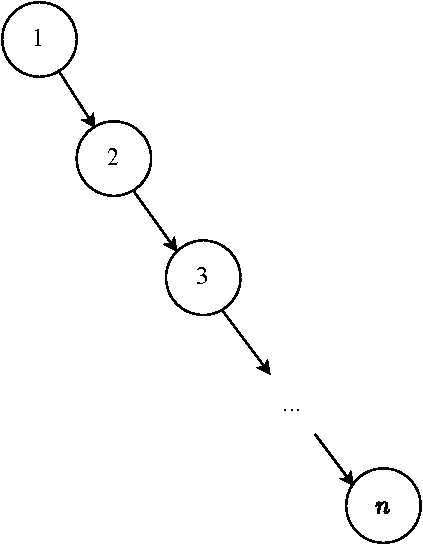
\includegraphics[scale=0.5]{img/unbalanced}
  \caption{unbalanced tree}
  \label{fig:unbalanced-tree}
\end{figure}

\begin{Exercise}
\Question{For a big address entry list in lexicographic order, one may want to speed up building the address book with two concurrent tasks: one reads from the head; the other from the tail, till they meet at some middle point. What does the binary search tree look like? What if split the list into multiple sections to scale the concurrency?}
\Question{Find more cases to exploit a binary search tree, for example in \cref{fig:unbalanced-trees}.}
\end{Exercise}

\begin{figure}[htbp]
  \centering
  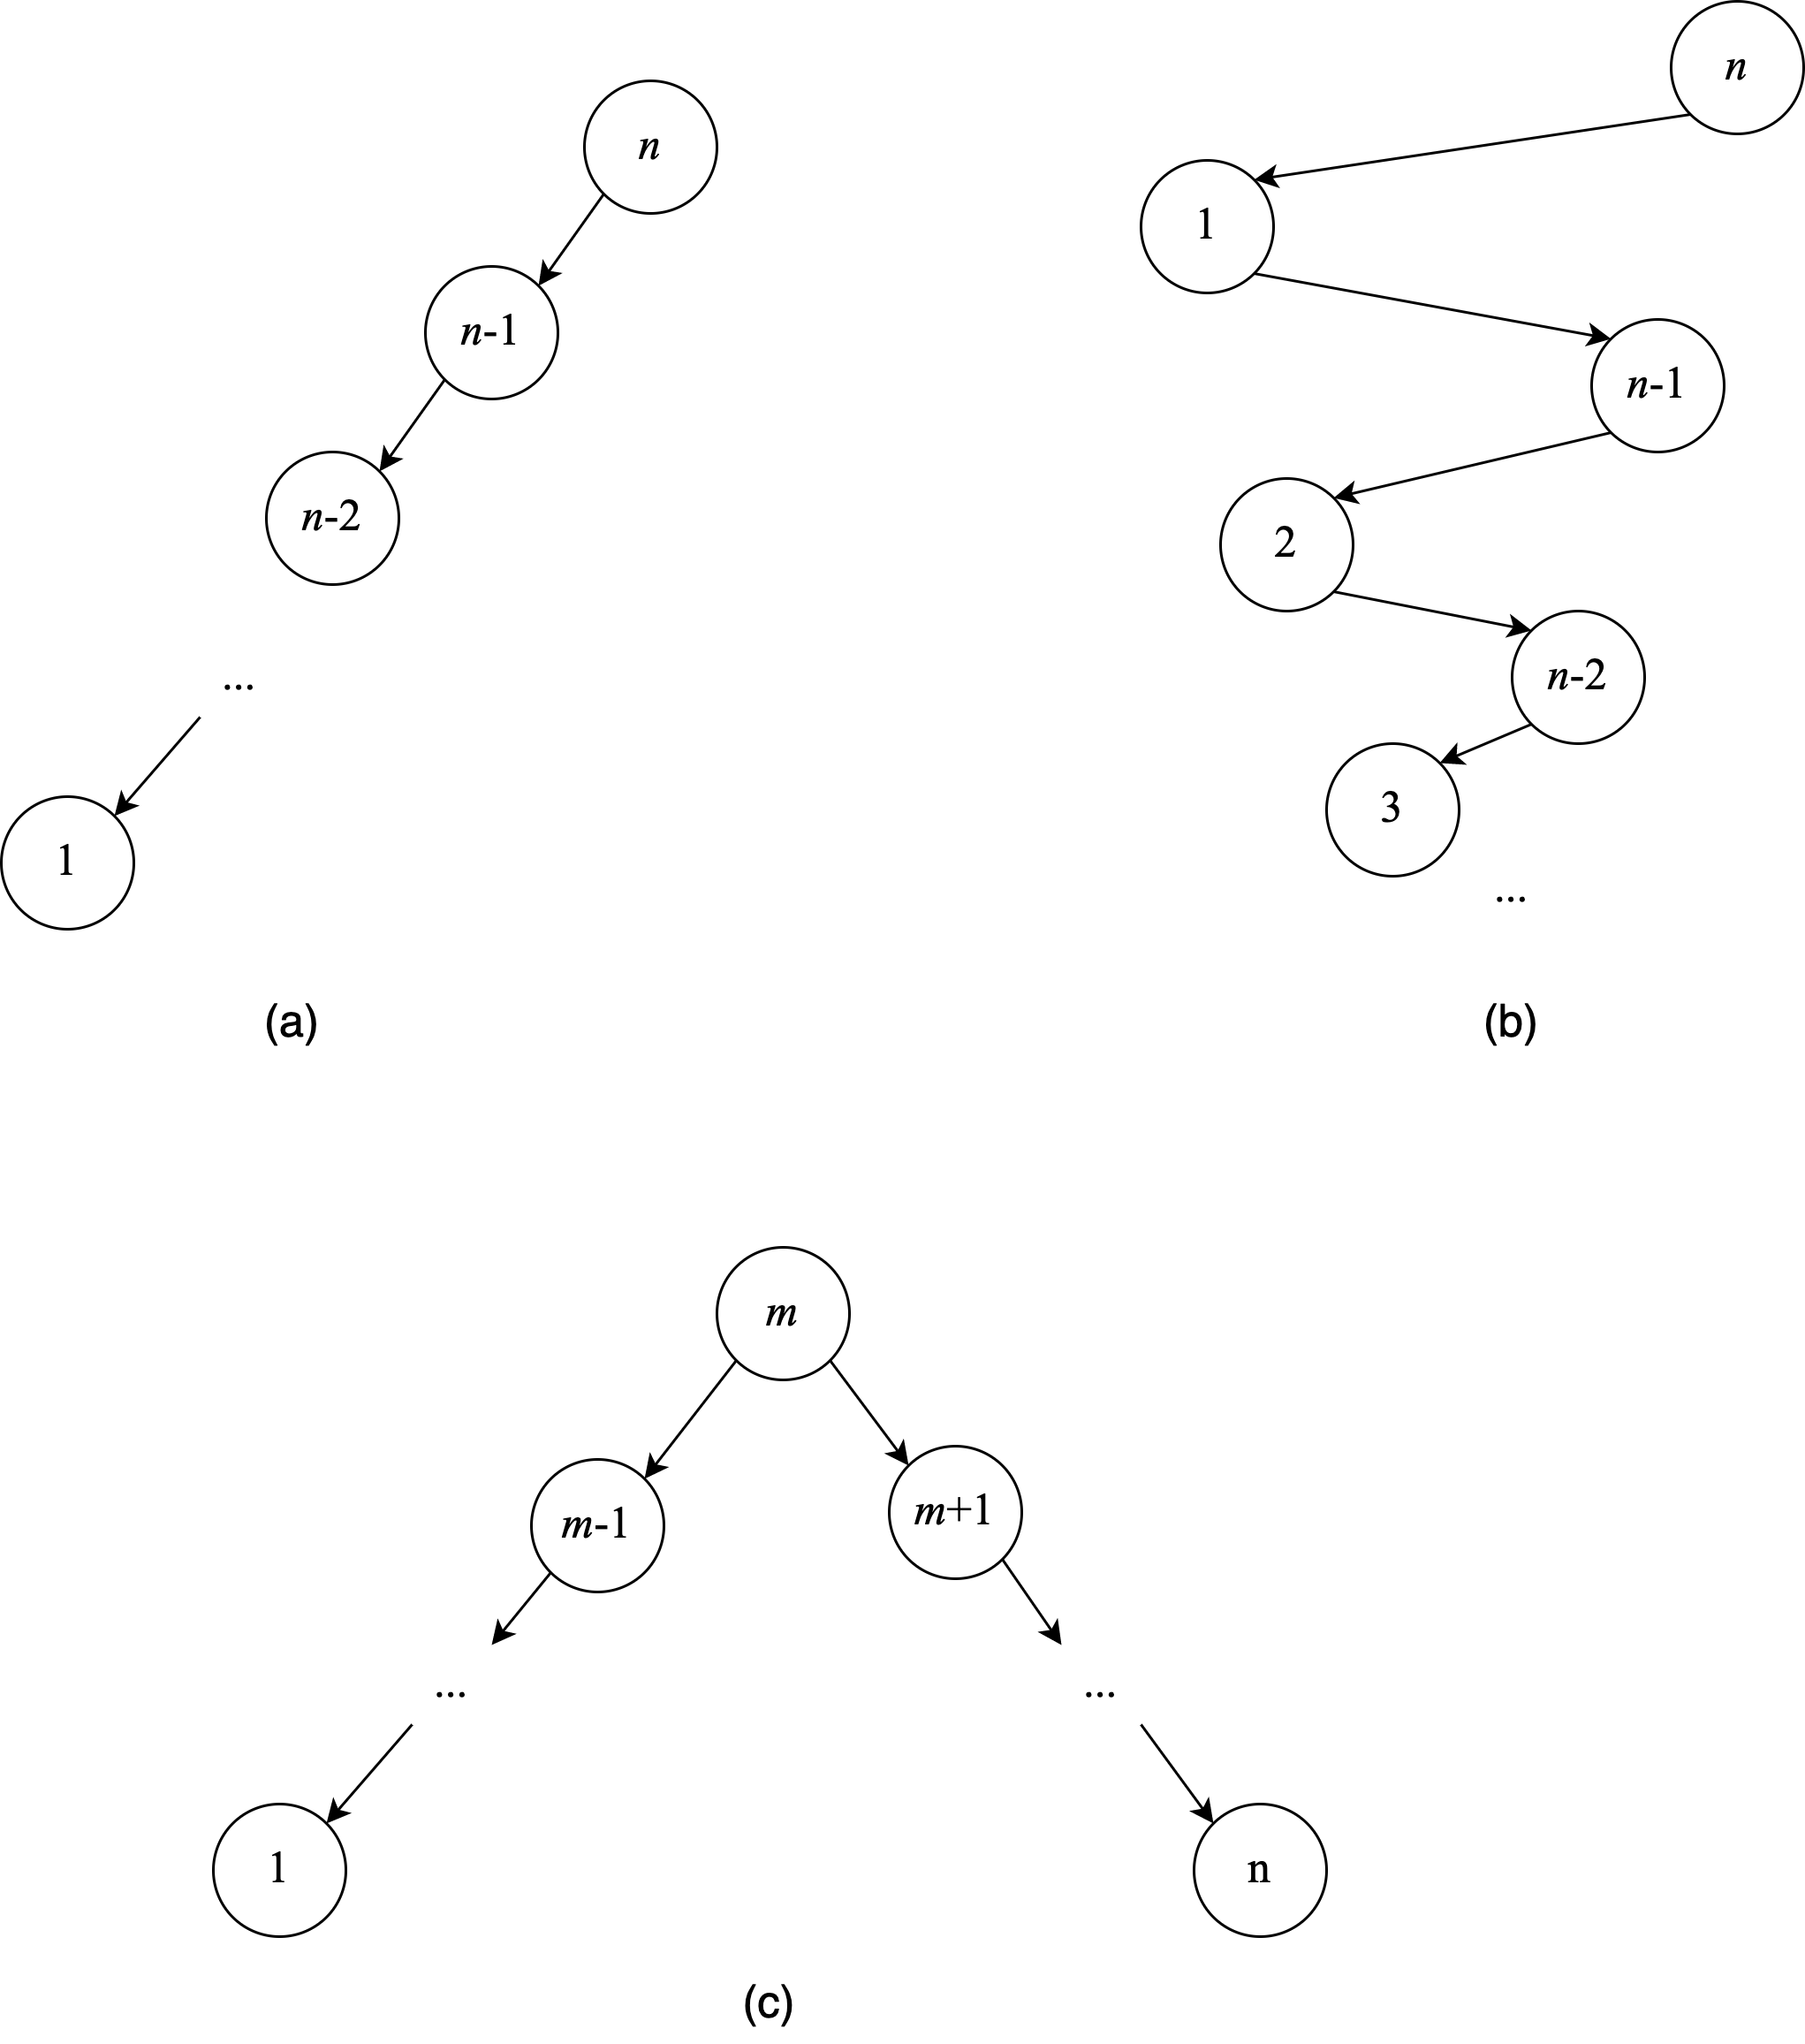
\includegraphics[scale=0.5]{img/unbalanced-trees}
  \caption{Unbalanced trees}
  \label{fig:unbalanced-trees}
\end{figure}

\section{Balance}
\index{tree rotation}

To avoid extremely unbalanced case, we can shuffle the input(\cref{sec:bst-random-build}), however, when user enter input interactively, we can not randomize it. Most tree balancing solutions rely on the rotation operation. Rotation changes the tree structure while maintain the elements ordering. This chapter introduces the red-black tree, a popular self-balancing binary search tree. Next chapter is about AVL tree, another self-balanced tree. Chapter 8 introduces the splay tree. It adjusts the tree in steps. There are multiple binary search trees have the same in-order traverse result. \Cref{fig:tree-rotation} shows the tree rotation. We can define them with pattern matching:

\begin{figure}[htbp]
   \centering
   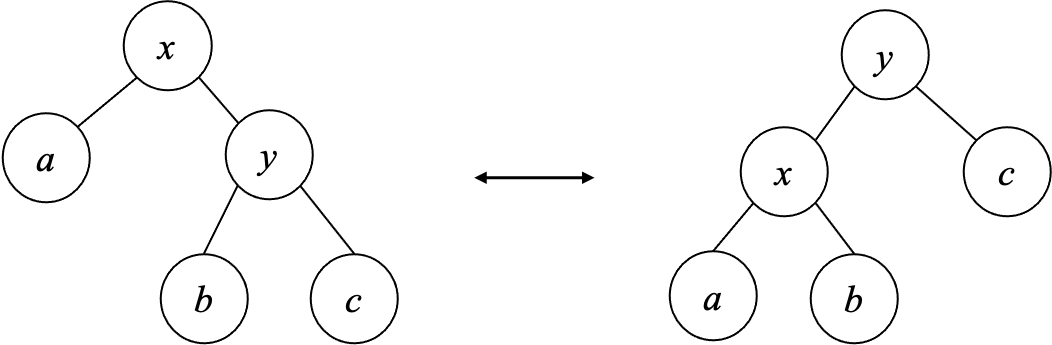
\includegraphics[scale=0.4]{img/tree-rotation}
   \caption{`left rotate' and `right rotate'.}
   \label{fig:tree-rotation}
\end{figure}

\be
\begin{array}{rcl}
rotate_l\ (a, x, (b, y, c)) & = & ((a, x, b), y, c)) \\
rotate_l\ T & = & T \\
\end{array}
\ee

and

\be
\begin{array}{rcl}
rotate_r\ ((a, x, b), y, c) & = & (a, x, (b, y, c)) \\
rotate_r\ T & = & T \\
\end{array}
\ee

Each second clause keeps the tree unchanged if the pattern does not match (for example, both sub-trees are empty). We can also implement tree rotation imperatively. We need re-assign sub-trees and parent reference. When rotate, we pass both the root $T$, and the node $x$ as parameters:

\begin{algorithmic}[1]
\Function{Left-Rotate}{$T, x$}
  \State $p \gets$ \Call{Parent}{$x$}
  \State $y \gets$ \Call{Right}{$x$} \Comment{assume $y \ne$ NIL}
  \State $a \gets$ \Call{Left}{$x$}
  \State $b \gets$ \Call{Left}{$y$}
  \State $c \gets$ \Call{Right}{$y$}
  \State \Call{Replace}{$x, y$}  \Comment{replace node $x$ with $y$}
  \State \Call{Set-Subtrees}{$x, a, b$} \Comment{Set $a, b$ as the sub-trees of $x$}
  \State \Call{Set-Subtrees}{$y, x, c$} \Comment{Set $x, c$ as the sub-trees of $y$}
  \If{$p = $ NIL}  \Comment{$x$ was the root}
    \State $T \gets y$
  \EndIf
  \State \Return $T$
\EndFunction
\end{algorithmic}

The \textproc{Right-Rotate} is symmetric, we leave it as exercise. The \textproc{Replace}($x$, $y$) uses node $y$ to replace $x$:

\begin{algorithmic}[1]
\Function{Replace}{$x, y$}
  \State $p \gets$ \Call{Parent}{$x$}
  \If{$p$ = NIL} \Comment{$x$ is the root}
    \If{$y \ne$ NIL}
           \Call{Parent}{$y$} $\gets$ NIL
    \EndIf
  \ElsIf{\Call{Left}{$p$} $= x$}
    \State \Call{Set-Left}{$p$, $y$}
  \Else
    \State \Call{Set-Right}{$p$, $y$}
  \EndIf
  \State \Call{Parent}{$x$} $\gets$ NIL
\EndFunction
\end{algorithmic}

Procedure \textproc{Set-Subtrees}($x, L, R$) assigns $L$ as the left, and $R$ as the right sub-trees of $x$:

\begin{algorithmic}[1]
\Function{Set-Subtrees}{$x, L, R$}
  \State \Call{Set-Left}{$x, L$}
  \State \Call{Set-Right}{$x, R$}
\EndFunction
\end{algorithmic}

It further calls \textproc{Set-Left} and \textproc{Set-Right} to set the two sub-trees:

\begin{algorithmic}[1]
\Function{Set-Left}{$x, y$}
  \State \Call{Left}{$x$} $\gets y$
  \If{$y \ne$ NIL}
    \Call{Parent}{$y$} $\gets x$
  \EndIf
  \EndFunction

\Statex

\Function{Set-Right}{$x, y$}
  \State \Call{Right}{$x$} $\gets y$
  \If{$y \ne$ NIL}
    \Call{Parent}{$y$} $\gets x$
  \EndIf
\EndFunction
\end{algorithmic}

We can see how pattern matching simplifies the tree rotation. Based on this idea, Okasaki developed the purely functional algorithm for red-black tree in 1995\cite{okasaki}.

\begin{Exercise}
\Question{Implement the \textproc{Right-Rotate}.}
\end{Exercise}

\section{Definition}
\index{red-black tree}

A red-black tree is a self-balancing binary search tree\cite{wiki-rbt}. It is equivalent to 2-3-4 tree\footnote{Chapter 7, B-tree. For any 2-3-4 tree, there is at least one red-black tree has the same ordered data.}. By coloring the node red or black, and performing rotation, red-black tree provides an efficient way to keep the tree balanced. On top of the binary search tree definition, we label the node with a color. We say it is a red-black tree if the coloring satisfies the following 5 rules(\cite{CLRS} pp273):

\index{red-black tree!red-black properties}
\begin{enumerate}
\item Every node is either red or black.
\item The root is black.
\item Every NIL node is black.
\item If a node is red, then both sub-trees are black.
\item For every node, all paths from it to descendant leaves contain the same number of black nodes.
\end{enumerate}

Why do they keep the red-black tree balanced? The key point is that, the longest path from the root to leaf can not exceed 2 times of the shortest path. Consider rule 4, there can not be any two adjacent red nodes. Hence the shortest path only contains black nodes. Any longer path must have red ones. In addition, rule 5 ensures all paths have the same number of black nodes. So as to the root. It eventually ensures any path can't exceed 2 times of the others\cite{wiki-rbt}. \Cref{fig:rbt-example-with-nil} gives an example of red-black tree.

\begin{figure}[htbp]
  \centering
  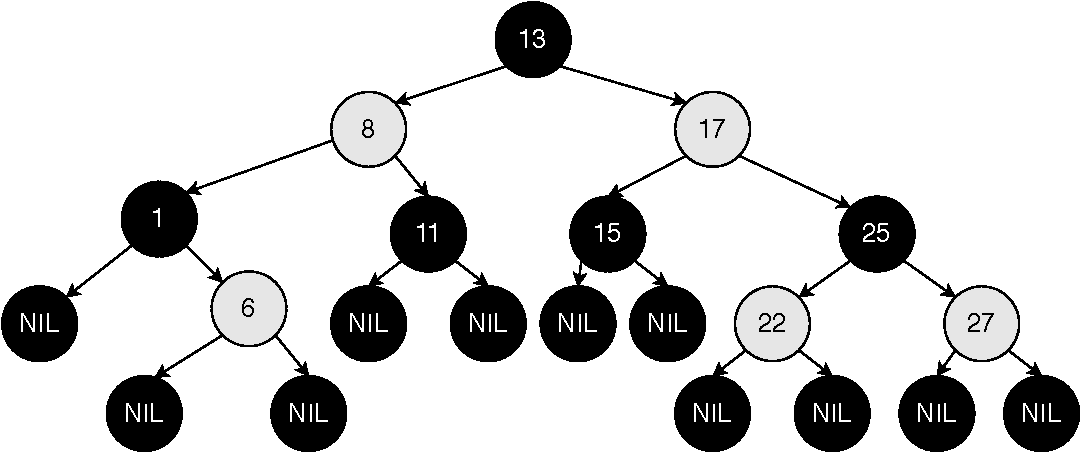
\includegraphics[scale=0.35]{img/rbt-example-with-nil}
  \caption{A red-black tree}
  \label{fig:rbt-example-with-nil}
\end{figure}

As all NIL nodes are black, we can hide them as shown in \cref{fig:rbt-example}. All operations including $lookup$, $\min/\max$, are same as the binary search tree. However, the $insert$ and $delete$ are special, as we need maintain the coloring rules. Below example program adds the color variable atop binary search tree definition. Denote the empty tree as $\nil$, the none empty tree as $(c, l, k,, r)$, where $c$ is the color (red/black), $k$ is the element, $l$ and $r$ are left and right sub-trees.

\begin{figure}[htbp]
  \centering
  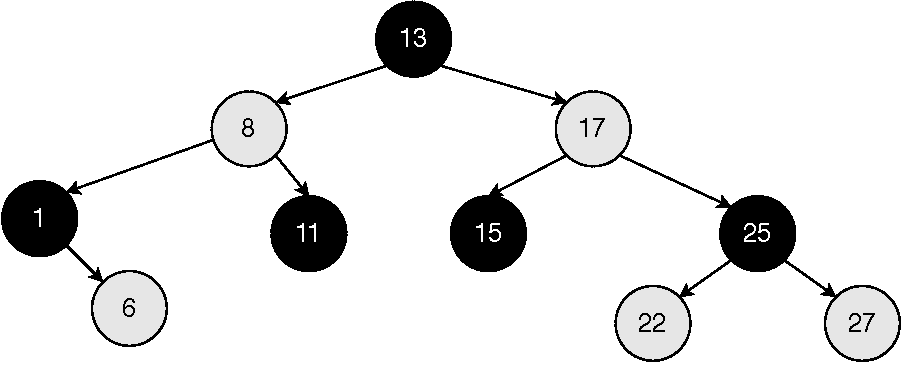
\includegraphics[scale=0.4]{img/rbt-example}
  \caption{Hide the NIL nodes}
  \label{fig:rbt-example}
\end{figure}

\begin{Haskell}
data Color = R | B
data RBTree a = Empty | Node Color (RBTree a) a (RBTree a)
\end{Haskell}

\begin{Exercise}\label{ex:rbt-bounds}
\Question{Prove the height $h$ of a red-black tree of $n$ nodes is at most $2 \lg (n+1)$}
\end{Exercise}

\begin{Answer}[ref = {ex:rbt-bounds}]
\Question{Prove the height $h$ of a red-black tree of $n$ nodes is at most $2 \lg (n+1)$

We first define the number of black nodes on any path from, but not including, a node $x$ down to a leaf the \textbf{black-height} of the node, denoted $bh(x)$. By property 5, all descending paths from the node have the same number of black nodes, hence the black-height is well defined. Particularly, we define the black-height of a red-black tree to be the black-height of its root.

\begin{proof}
We first prove that any sub-tree rooted at $x$ contains at least $2^{bh(x)} - 1$ nodes. Apply mathematical induction on the height of $x$. if $h(x) = 0$, then $x$ is NIL. It contains at least $2^0 - 1 = 0$ nodes. Consider a branch node $x$, The black-height of its two sub-trees is either $bh(x)$ (the root of the sub-tree is black) or $bh(x) - 1$ (the root of the sub-tree is red). Since the height of the sub-tree of $x$ is less than $h(x)$, from the induction hypothesis, each sub-tree contains at least $2^{bh(x) - 1} - 1$ nodes. Hence the sub-tree rooted at $x$ contains at least: $2(2^{bh(x) - 1} - 1) + 1 = 2^{bh(x)} - 1$ nodes.

Let the height of the tree be $h$, according to property 4, there are not adjacent red nodes. There are more than half black nodes on any path from the root to the leaf. Hence the black-height of the tree is at least $h/2$. We have:

\[
n \geq 2^{h/2} - 1 \Rightarrow 2^{h/2} \leq n + 1
\]

Take logarithm on both sides: $h/2 \leq \lg (n + 1)$, i.e., $h \leq 2 \lg (n + 1)$.
\end{proof}
}
\end{Answer}

\section{Insert}
\index{red-black tree!insert}

The $insert$ operation takes two steps. The first step is as same as the binary search tree. The second step if to resume the coloring if it becomes unbalanced. We always color the new element red unless it is the root. Hence don't break any coloring rules except the 4-th. Because it may bring two adjacent red nodes. There are 4 cases violate rule 4. They share the same structure after fixing\cite{okasaki} as shown in \cref{fig:insert-fix}.

\begin{figure}[htbp]
  \centering
  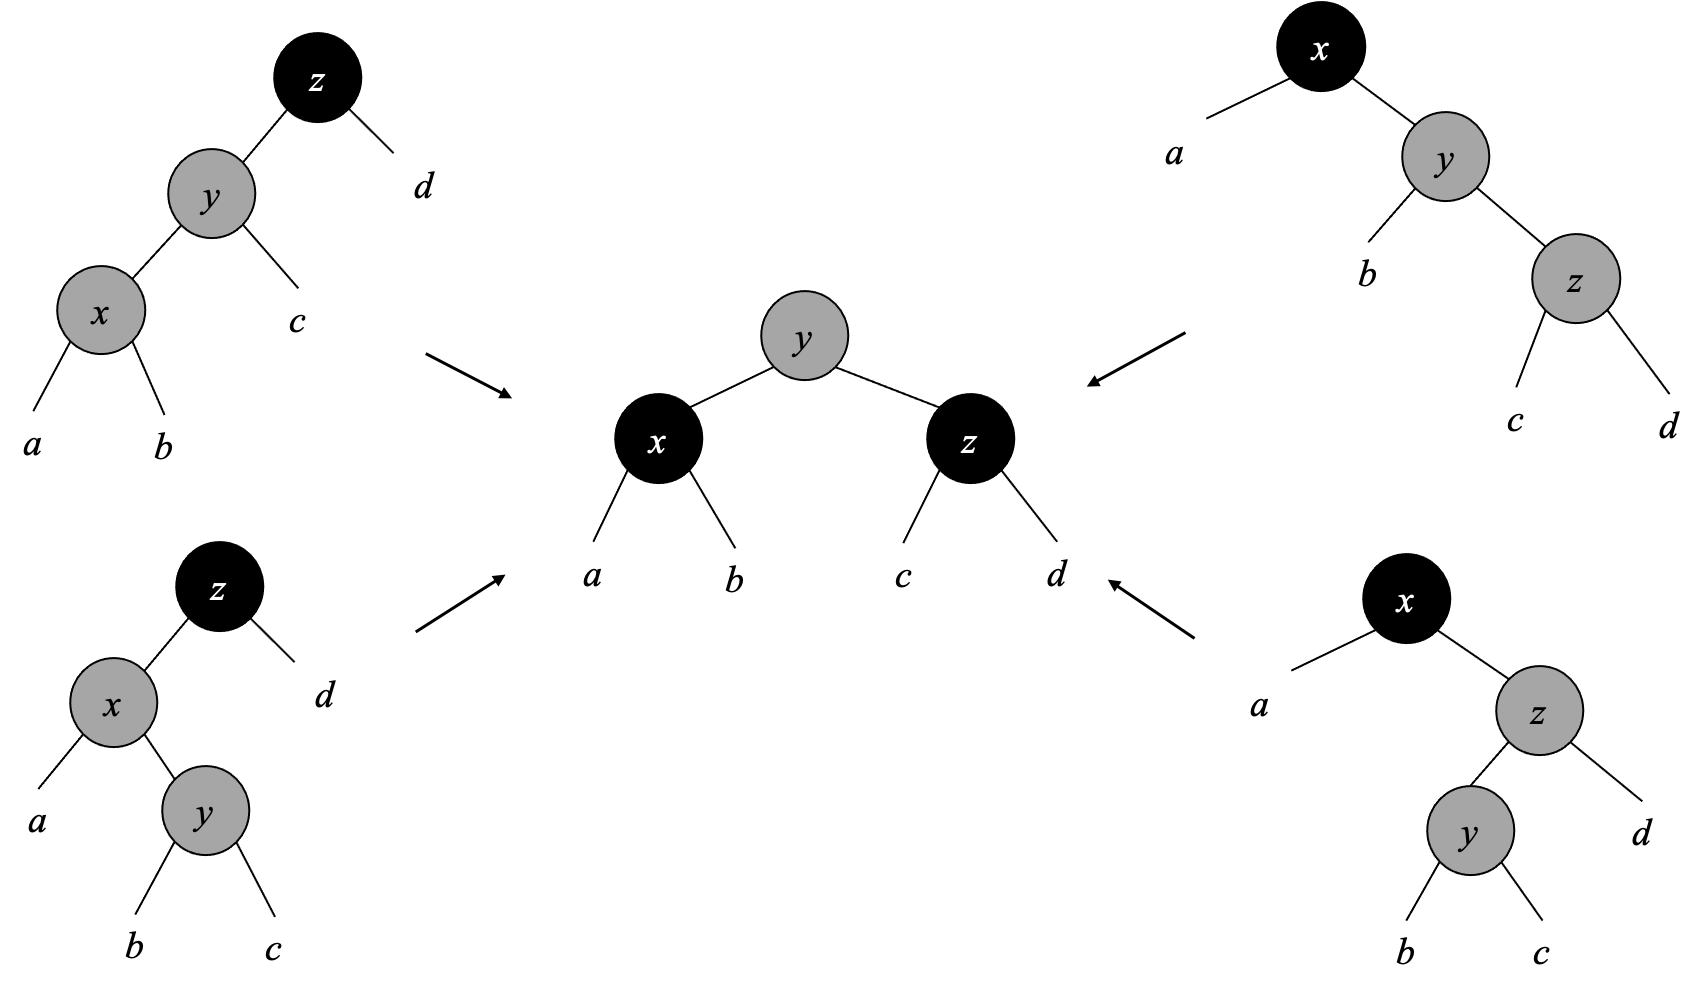
\includegraphics[scale=0.4]{img/insert-fix}
  \caption{Fix 4 cases to the same structure.}
  \label{fig:insert-fix}
\end{figure}

All 4 transformations move the redness one level up. When fix recursively bottom-up, it may color the root red, hence violate rule 2. We need revert the root black finally. With pattern matching, define a $balance$ function to fix the coloring. Denote the color as $\mathcal{C}$ with values black $\mathcal{B}$, and red $\mathcal{R}$.

\be
\begin{array}{rcl}
%\text{up left:} & & \\
balance\ \mathcal{B}\ (\mathcal{R}, (\mathcal{R}, a, x, b), y, c)\ z\ d & = & (\mathcal{R}, (\mathcal{B}, a, x, b), y, (\mathcal{B}, c, z, d)) \\
%\text{up right:} & & \\
balance\ \mathcal{B}, (\mathcal{R}, a, x, (\mathcal{R}, b, y, c))\ z\ d  & = & (\mathcal{R}, (\mathcal{B}, a, x, b), y, (\mathcal{B}, c, z, d)) \\
%\text{bottom left:} & & \\
balance\ \mathcal{B}\ a\ x\ (\mathcal{R}, b, y, (\mathcal{R}, c, z, d)) & = & (\mathcal{R}, (\mathcal{B}, a, x, b), y, (\mathcal{B}, c, z, d))  \\
%\text{bottom right:} & & \\
balance\ \mathcal{B}\ a\ x\ (\mathcal{R}, (\mathcal{R}, b, y, c), z, d) & = & (\mathcal{R}, (\mathcal{B}, a, x, b), y, (\mathcal{B}, c, z, d))  \\
%\text{otherwise:} & & \\
balance\ T & = & T \\
\end{array}
\ee

If none of the 4 patterns matches, we leave the tree unchanged. Define the red-black tree $insert$ as: $insert\ x\ T = makeBlack\ (ins\ x\ T)$, or in Curried form:

\be
insert x = makeBlack \circ ins\ x
\ee

Where:

\be
\begin{array}{rcl}
ins\ x\ \nil\ & = & (\mathcal{R}, \nil, x, \nil) \\
ins\ x\ (\mathcal{C}, l, k, r) & = & \begin{cases}
  x < k: & balance\ \mathcal{C}\ (ins\ x\ l)\ k\ r \\
  x > k: & balance\ \mathcal{C}\ l\ k\ (ins\ x\ r) \\
  \end{cases}
\end{array}
\ee

If the tree is empty, we create a red leaf of $x$; otherwise, compare $x$ and $k$, recursively insert $x$ to a sub-tree. After that, call $balance$ to fix the coloring, finally force the root to be black.

\be
makeBlack\ (\mathcal{C}, l, k, r) = (\mathcal{B}, l, k, r)
\ee

Below is the example program:

\begin{Haskell}
insert x = makeBlack . (ins x) where
    ins x Empty = Node R Empty x Empty
    ins x (Node color l k r)
        | x < k     = balance color (ins x l) k r
        | otherwise = balance color l k (ins x r)
    makeBlack (Node _ l k r) = Node B l k r

balance B (Node R (Node R a x b) y c) z d = Node R (Node B a x b) y (Node B c z d)
balance B (Node R a x (Node R b y c)) z d = Node R (Node B a x b) y (Node B c z d)
balance B a x (Node R b y (Node R c z d)) = Node R (Node B a x b) y (Node B c z d)
balance B a x (Node R (Node R b y c) z d) = Node R (Node B a x b) y (Node B c z d)
balance color l k r = Node color l k r
\end{Haskell}

We skip to handle the duplicated keys. If the key already exists, we can overwrite, drop, or store the values in a list (\cite{CLRS}, pp269). \Cref{fig:insert-example} shows two red-black trees built from sequence 11, 2, 14, 1, 7, 15, 5, 8, 4 and 1, 2, ..., 8. The second example is well balanced even for ordered input.

\begin{figure}[htbp]
  \centering
  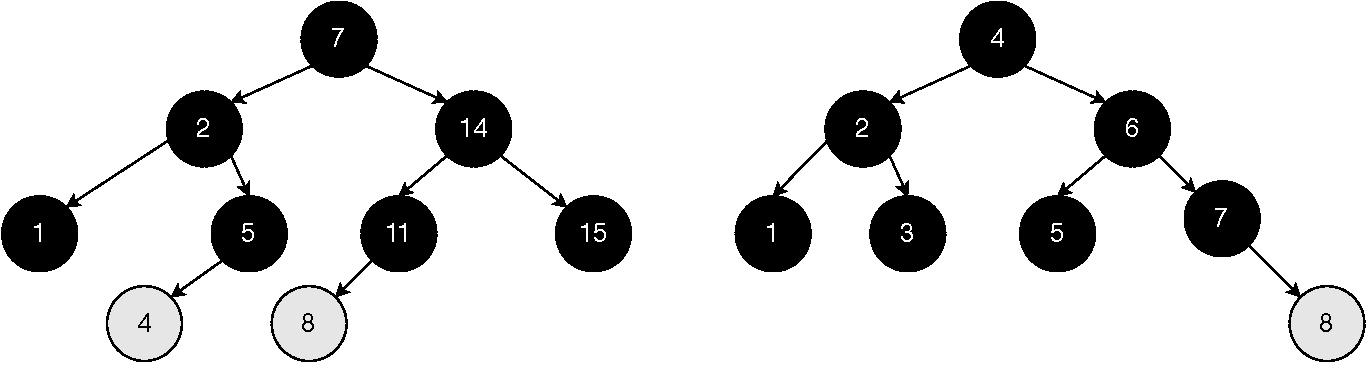
\includegraphics[scale=0.35]{img/insert-haskell}
  \caption{Red-black tree examples}
  \label{fig:insert-example}
\end{figure}

The $insert$ performs top-down recursive fixing. It is bound to $O(h)$ time, where $h$ is the height. As the red-black tree coloring rules are maintained, $h$ is logarithm to $n$, the number of elements. The overall performance is $O(\lg n)$.

\begin{Exercise}\label{ex:rbt-insert-wo-pm}
\Question{Implement the $insert$ without pattern matching, handle the 4 cases separately.}
\end{Exercise}

\begin{Answer}[ref = {ex:rbt-insert-wo-pm}]
\Question{Implement the $insert$ without pattern matching, handle the 4 cases separately.

\begin{Bourbaki}
Node<T> insert(Node<T> t, T x) = makeBlack(ins(t, x))

Node<T> makeBlack(Node<T> t) {
    t.color = Color.BLACK
    return t
}

Node<T> ins(Node<T> t, T x) {
    if t == null then return Node(null, x, null, Color.BLACK)
    return if x < t.key
           then balance(t.color, ins(t.left, x), t.key, t.right)
           else balance(t.color, t.left, t.key, ins(t.right, x))
}

Node<T> balance(Color c, Node<T> l, T k, Node<T> r) {
    return if c == Color.BLACK {
        if isRed(l) and isRed(l.left) {
            Node(Node(l.left.left, l.left.key, l.left.right, Color.BLACK),
                 l.key,
                 Node(l.right, k, r, Color.BLACK),
                 Color.RED)
        } else if isRed(l) and isRed(l.right) {
            Node(Node(l.left, l.key, l.right.left, Color.BLACK),
                 l.right.key,
                 Node(l.right.right, k, r, Color.BLACK),
                 Color.RED)
        } else if isRed(r) and isRed(r.right) {
            Node(Node(l, k, r.left, Color.BLACK),
                 r.key,
                 Node(r.left.right, r.right.key, r.right.right, Color.BLACK),
                 Color.RED)
        } else if isRed(r) and isRed(r.left) {
            Node(Node(l, k, r.left.left, Color.BLACK),
                 r.left.key,
                 Node(r.left.right, r.key, r.right, Color.BLACK),
                 Color.RED)
        } else {
            Node(l, k, r, c)
        }
    } else {
        Node(l, k, r, c)
    }
}

Bool isRed(Node<T> t) = (t != null and t.color == Color.RED)
\end{Bourbaki}
}
\end{Answer}

\section{Delete}
\index{red-black tree!delete}

Delete is more complex than insert. We can simplify the recursive implementation with pattern matching\footnote{Actually, we reuse the unchanged part to rebuild the tree in purely functional settings, known as the `persist' feature}. There are alternative implementation to mimic delete. Build a read-only tree for frequently looking up\cite{okasaki-blog}. When delete a node, mark it with a flag, and trigger tree rebuilding if such nodes exceeds 50\%. Delete may also violate the red-black tree coloring rules, hence need fixing. The violation only happens when delete a black node according to rule 5. The black nodes along the path decreases by one, causing not all paths contain the same number of black nodes. To resume the blackness, we introduce a special `doubly-black' node(\cite{CLRS}, pp290). Such a node is counted as 2 black nodes. When delete a black node $x$, move the blackness up to parent or down to a sub-tree. Let node $y$ accept the blackness. If $y$ was red, turn it black; if $y$ was already black, turn it `doubly-black' as $\mathcal{B}^2$. Below example program adds the `doubly-black' color.

\begin{Haskell}
data Color = R | B | BB
data RBTree a = Empty | BBEmpty | Node Color (RBTree a) a (RBTree a)
\end{Haskell}

Because ever NIL is black, when push the blackness down to NIL, it becomes `doubly-black' empty (\texttt{BBEmpty}, or bold $\pmb{\varnothing}$). The first step is normal binary search tree delete; then as the second step, if cut a black node off, shift the blackness, and fix the coloring.

\be
delete\ x = makeBlack \circ del\ x
\ee

This is Curried definition. When delete a singleton tree, it becomes empty. To cover this case, we modify $makeBlack$ as below:

\be
\begin{array}{rcl}
makeBlack\ \nil & = & \nil \\
makeBlack\ (\mathcal{C}, l, k, r) & = & (\mathcal{B}, l, k, r) \\
\end{array}
\ee

Where $del$ accepts $x$ and the tree:

\be
\resizebox{\linewidth}{!}{\ensuremath{
\begin{array}{rcl}
del\ x\ \nil\ & = & \nil \\
del\ x\ (\mathcal{C}, l, k, r) & = & \begin{cases}
  x < k: & fixB^2(\mathcal{C}, (del\ x\ l), k, r) \\
  x > k: & fixB^2(\mathcal{C}, l, k, (del\ x\ r)) \\
  x = k: & \begin{cases}
    l = \nil: & \text{if}\ \mathcal{C} = \mathcal{B}\ \text{then}\ shiftB\ r\ \text{else}\ r \\
    r = \nil: & \text{if}\ \mathcal{C} = \mathcal{B}\ \text{then}\ shiftB\ l\ \text{else}\ l \\
    \text{otherwise}: & fixB^2(\mathcal{C}, l, m, (del\ m\ r)), \text{where}: m = min(r) \\
  \end{cases}
\end{cases}
\end{array}
}}
\ee

When the tree is empty, the result is $\nil$; otherwise, we compare $x$ and $k$. If $x < k$, we recursively delete from left; otherwise delete from right. Because the recursive result may contain doubly-black node, we apply $fixB^2$ to fix. When $x = k$, we locate the node to cut. If either sub-tree is empty, we replace the node with the none empty sub-tree, then shift the blackness if the node is black. If neither sub-tree is empty, we cut the minimum $m = \min\ r$ off, and use $m$ to replace $k$. To reserve the blackness, $shiftB$ makes a black node doubly-black, and forces it black for other cases. It flips doubly-black to normal black when applied twice.

\be
\begin{array}{rcl}
shiftB\ (\mathcal{B}, l, k, r) & = & (\mathcal{B}^2, l, k, r) \\
shiftB\ (\mathcal{C}, l, k, r) & = & (\mathcal{B}, l, k, r) \\
shiftB\ \nil & = & \pmb{\nil} \\
shiftB\ \pmb{\nil} & = & \nil \\
\end{array}
\ee

Below is the example program (except the doubly-black fixing part).

\begin{Haskell}
delete x = makeBlack . (del x) where
    del x Empty = Empty
    del x (Node color l k r)
        | x < k = fixDB color (del x l) k r
        | x > k = fixDB color l k (del x r)
        | isEmpty l = if color == B then shiftBlack r else r
        | isEmpty r = if color == B then shiftBlack l else l
        | otherwise = fixDB color l m (del m r) where m = min r
    makeBlack (Node _ l k r) = Node B l k r
    makeBlack _ = Empty

isEmpty Empty = True
isEmpty _ = False

shiftBlack (Node B l k r) = Node BB l k r
shiftBlack (Node _ l k r) = Node B  l k r
shiftBlack Empty = BBEmpty
shiftBlack BBEmpty = Empty
\end{Haskell}

The $fixB^2$ function eliminates the doubly-black by rotation and re-coloring. The doubly-black node can be branch node or empty $\pmb{\varnothing}$. There are three cases:

\textbf{Case 1}. {\em The sibling of the doubly-black node is black, and it has a red sub-tree.} We can fix this case with a rotation. There are 4 sub-cases, all can transform to the same pattern, as shown in \cref{fig:del-case1}.

\begin{figure}[htbp]
  \centering
  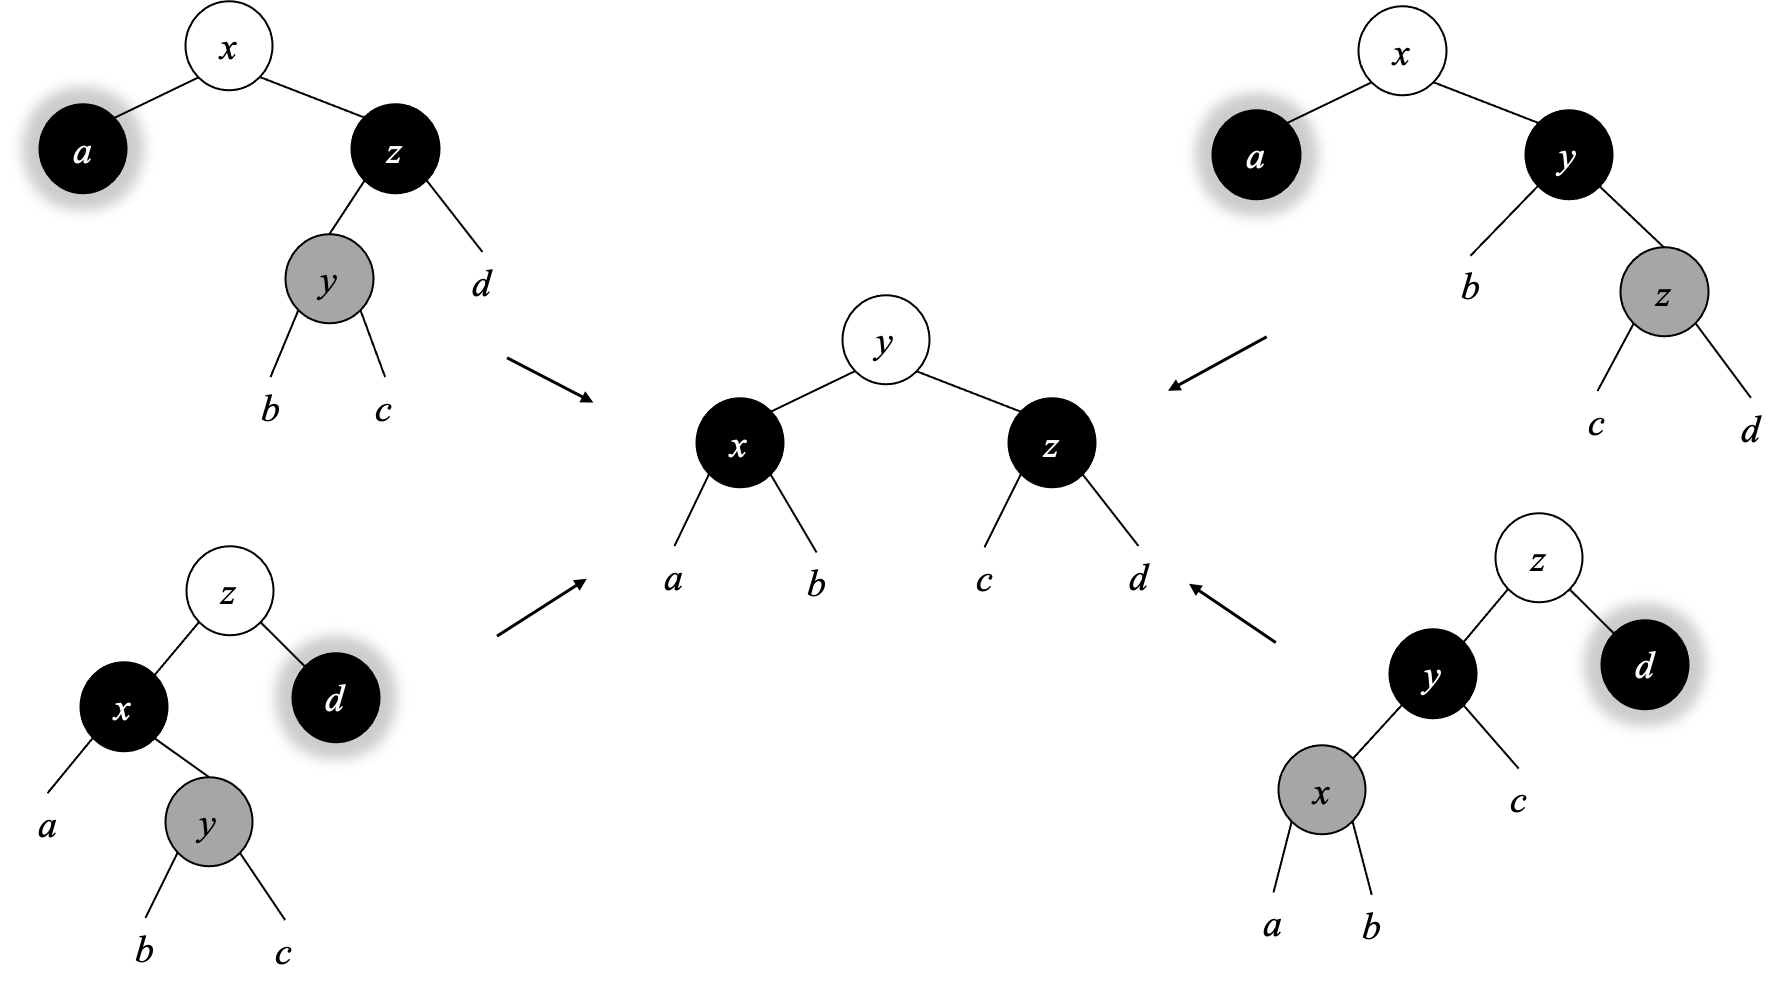
\includegraphics[scale=0.4]{img/del-case1}
  \caption{Transform 4 sub-cases to the same pattern}
  \label{fig:del-case1}
\end{figure}

\be
\resizebox{\textwidth}{!}{\ensuremath{
\begin{array}{rcl}
%\text{case 1 up left:} & & \\
fixB^2\ \mathcal{C}\ a_{\mathcal{B}^2}\ x\ (\mathcal{B}, (\mathcal{R}, b, y, c), z, d) & = & (\mathcal{C}, (\mathcal{B}, shiftB(a), x, b), y, (\mathcal{B}, c, z, d)) \\
%\text{case 1 up right:} & & \\
fixB^2\ \mathcal{C}\ a_{\mathcal{B}^2}\ x\ (\mathcal{B}, b, y, (\mathcal{R}, c, z, d)) & = & (\mathcal{C}, (\mathcal{B}, shiftB(a), x, b), y, (\mathcal{B}, c, z, d)) \\
%\text{case 1 bottom left:} & & \\
fixB^2\ \mathcal{C}\ (\mathcal{B}, a, x, (\mathcal{R}, b, y, c))\ z\ d_{\mathcal{B}^2} & = & (\mathcal{C}, (\mathcal{B}, a, x, b), y, (\mathcal{B}, c, z, shiftB(d))) \\
%\text{case 1 bottom right:} & & \\
fixB^2\ \mathcal{C}\ (\mathcal{B}, (\mathcal{R}, a, x, b), y, c)\ z\ d_{\mathcal{B}^2} & = & (\mathcal{C}, (\mathcal{B}, a, x, b), y, (\mathcal{B}, c, z, shiftB(d))) \\
\end{array}
}}
\label{eq:db-case-1}
\ee

Where $a_{\mathcal{B}^2}$ means node $a$ is doubly-black.

\textbf{Case 2}. {\em The sibling of the doubly-black is red.} We can rotate the tree to turn it into case 1 or 3, as shown in \cref{fig:del-case2}. We add this fixing as additional 2 rows in \cref{eq:db-case-1}:

\begin{figure}[htbp]
  \centering
  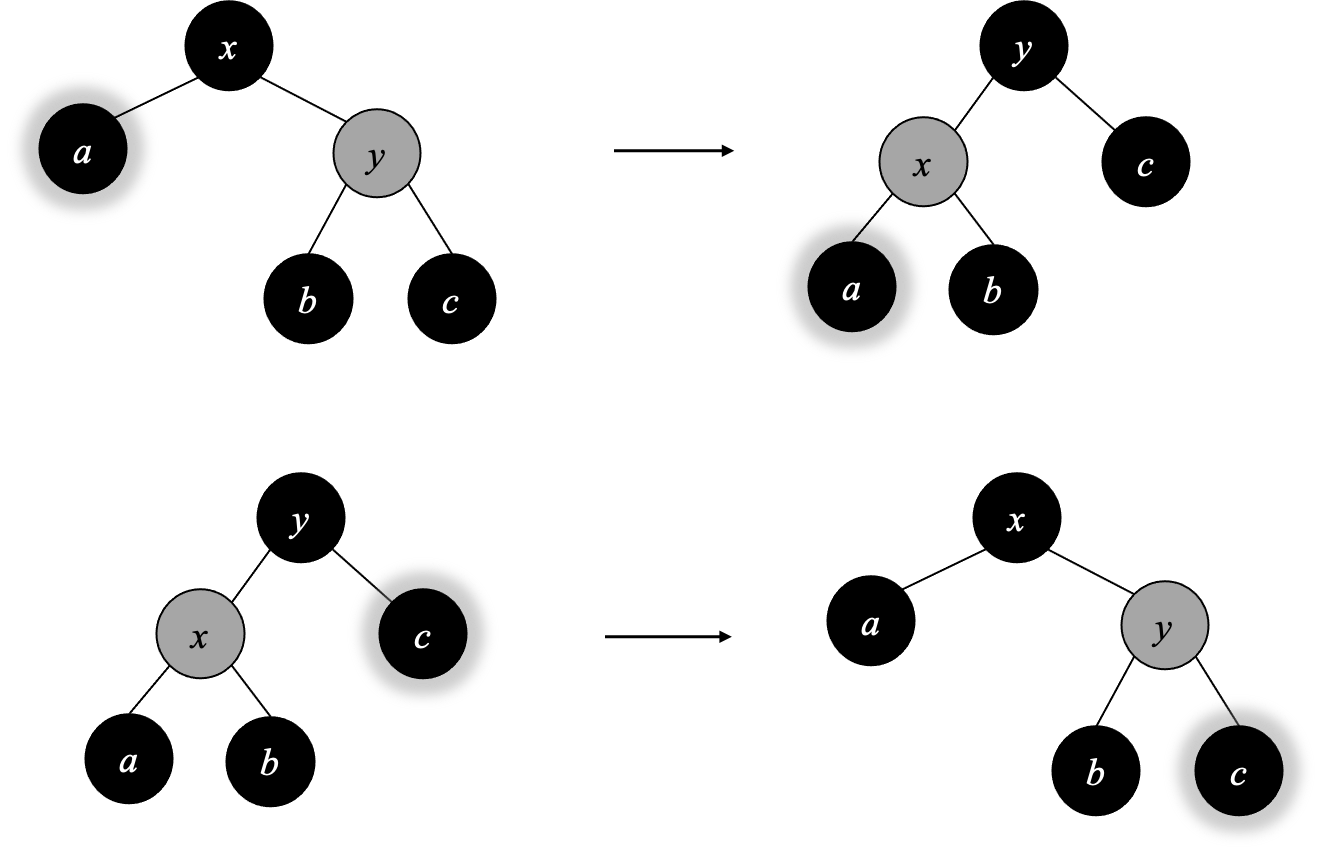
\includegraphics[scale=0.4]{img/del-case2}
  \caption{The sibling of the doubly-black is red.}
  \label{fig:del-case2}
\end{figure}

\be
%\resizebox{\textwidth}{!}{\ensuremath{
\begin{array}{rcl}
\text{...} & & \\
%\text{case 2 up:} & & \\
fixB^2\ \mathcal{B}\ a_{\mathcal{B}^2}\ x\ (\mathcal{R}, b, y, c) & = & fixB^2\ \mathcal{B}\ (fixB^2\ \mathcal{R}\ a\ x\ b)\ y\ c \\
%\text{case 2 bottom:} & & \\
fixB^2\ \mathcal{B}\ (\mathcal{R}, a, x, b)\ y\ c_{\mathcal{B}^2} & = & fixB^2\ \mathcal{B}\ a\ x\ (fixB^2\ \mathcal{R}\ b\ y\ c)
\end{array}
%}}
\label{eq:db-case-2}
\ee

\textbf{Case 3}. {\em The sibling of the doubly-black node, and its two sub-trees are all black.} In this case, we change the sibling to red, flip the doubly-black node to black, and propagate the doubly-blackness a level up to parent as shown in \cref{fig:del-case3}. There are two symmetric sub-cases. For the upper case, $x$ was either red or black. $x$ changes to black if it was red, otherwise changes to doubly-black; Same coloring changes to $y$ in the lower case. We add this fixing to \cref{eq:db-case-2}:

\begin{figure}[htbp]
  \centering
  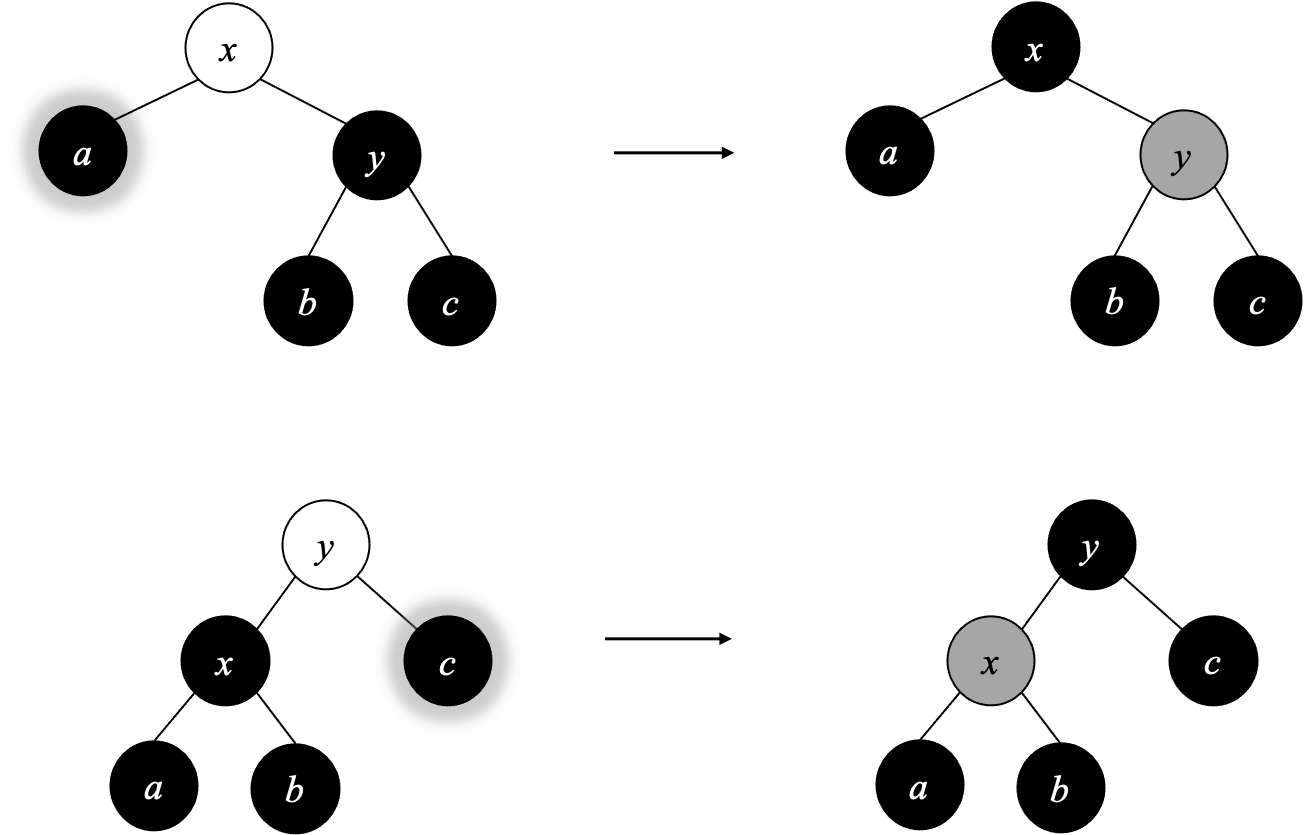
\includegraphics[scale=0.4]{img/del-case3}
  \caption{move the blackness up.}
  \label{fig:del-case3}
\end{figure}

\be
%\resizebox{\textwidth}{!}{\ensuremath{
\begin{array}{rcl}
\text{...} & & \\

fixB^2\ \mathcal{C}\ a_{\mathcal{B}^2}\ x\ (\mathcal{B}, b, y, c) & = & shiftB\ (\mathcal{C}, (shiftB\ a), x, (\mathcal{R}, b, y, c)) \\

fixB^2\ \mathcal{C}\ (\mathcal{B}, a, x, b)\ y\ c_{\mathcal{B}^2} & = & shiftB\ (\mathcal{C}, (\mathcal{R}, a, x, b), y, (shiftB\ c)) \\

fixB^2\ \mathcal{C}\ l\ k\ r\ & = & (\mathcal{C}, l, k, r) \\
\end{array}
%}}
\label{eq:db-case-3}
\ee

If none of the patterns match, the last row keeps the node unchanged. The doubly-black fixing is recursive. It terminates in two ways: One is \textbf{Case 1}, the doubly-black node is eliminated. Otherwise the blackness may move up till the root. Finally the we force the root be black. Below example program puts all three cases together:

\begin{Haskell}
fixDB color a@(Node BB _ _ _) x (Node B (Node R b y c) z d)
      = Node color (Node B (shiftBlack a) x b) y (Node B c z d)
fixDB color BBEmpty x (Node B (Node R b y c) z d)
      = Node color (Node B Empty x b) y (Node B c z d)
fixDB color a@(Node BB _ _ _) x (Node B b y (Node R c z d))
      = Node color (Node B (shiftBlack a) x b) y (Node B c z d)
fixDB color BBEmpty x (Node B b y (Node R c z d))
      = Node color (Node B Empty x b) y (Node B c z d)
fixDB color (Node B a x (Node R b y c)) z d@(Node BB _ _ _)
      = Node color (Node B a x b) y (Node B c z (shiftBlack d))
fixDB color (Node B a x (Node R b y c)) z BBEmpty
      = Node color (Node B a x b) y (Node B c z Empty)
fixDB color (Node B (Node R a x b) y c) z d@(Node BB _ _ _)
      = Node color (Node B a x b) y (Node B c z (shiftBlack d))
fixDB color (Node B (Node R a x b) y c) z BBEmpty
      = Node color (Node B a x b) y (Node B c z Empty)
fixDB B a@(Node BB _ _ _) x (Node R b y c)
      = fixDB B (fixDB R a x b) y c
fixDB B a@BBEmpty x (Node R b y c)
      = fixDB B (fixDB R a x b) y c
fixDB B (Node R a x b) y c@(Node BB _ _ _)
      = fixDB B a x (fixDB R b y c)
fixDB B (Node R a x b) y c@BBEmpty
      = fixDB B a x (fixDB R b y c)
fixDB color a@(Node BB _ _ _) x (Node B b y c)
      = shiftBlack (Node color (shiftBlack a) x (Node R b y c))
fixDB color BBEmpty x (Node B b y c)
      = shiftBlack (Node color Empty x (Node R b y c))
fixDB color (Node B a x b) y c@(Node BB _ _ _)
      = shiftBlack (Node color (Node R a x b) y (shiftBlack c))
fixDB color (Node B a x b) y BBEmpty
      = shiftBlack (Node color (Node R a x b) y Empty)
fixDB color l k r = Node color l k r
\end{Haskell}

The delete algorithm is bound to $O(h)$ time, where $h$ is the height of the tree. As red-black tree maintains the balance, $h = O(\lg n)$ for $n$ nodes.

\begin{Exercise}\label{ex:mark-rebuild}
\Question{Implement the `mark-rebuild' delete algorithm: mark the node as deleted without actually removing it. When the marked nodes exceed 50\%, rebuild the tree.}
\end{Exercise}

\begin{Answer}[ref = {ex:mark-rebuild}]
\Question{Implement the `mark-rebuild' delete algorithm: mark the node as deleted without actually removing it. When the marked nodes exceed 50\%, rebuild the tree.

We augment each key $x$ with a flag $a$ in the node. The type of the tree is $Tree\ (K, Bool)$. When insert $x$, call $insert\ (x, True)$ to mark the node active. When delete, flip $a$ to False, then count the active node number and trigger rebuild if exceeds half.

\[
delete\ x\ = rebuild \circ del\ x
\]

Where:

\[
\begin{array}{rcl}
del\ x\ \nil & = & \nil \\
del\ x\ (c, l, (k, a), r) & = & \begin{cases}
  x < k: & (c, del\ x\ l, (k, a), r) \\
  x > k: & (c, l, (k, a), del\ x\ r) \\
  x = k: & (c, l, (k, False), r) \\
\end{cases}
\end{array}
\]

Of there are more than half nodes are inactive, we convert the tree to a list, filter the active nodes and rebuild the tree.

\[
rebuild\ t = \begin{cases}
  size\ t < \dfrac{1}{2} (cap\ t): & (fromList \circ toList)\ t \\
  \text{otherwise}: & t
\end{cases}
\]

Where $toList$ traverse the tree and skip the deleted nodes:

\[
\begin{array}{rcl}
toList\ \nil & = & [\ ] \\
toList\ (c, l, (k, a), r) & = &
  \begin{cases}
    a: & toList\ l \doubleplus [k] \doubleplus toList\ r \\
    \text{otherwise}: & toList\ l \doubleplus toList\ r \\
  \end{cases}
\end{array}
\]

To avoid traverse the entire tree every time when count the nodes, we save the tree capacity and size in each node. Extend the type of the tree to $Tree\ (K, Bool, Int, Int)$, and define $node$ as:

\[
\begin{array}{rcl}
node\ \nil & = & \nil \\
node\ c\ l\ (k, a, \_, \_)\ r & = & (c, l, (k, a, sz, ca), r) \\
\end{array}
\]

Where:

\[
\begin{cases}
sz = size\ l + size\ r + (\text{if}\ a\ \text{then}\ 1\ \text{else}\ 0) \\
ca = 1 + cap\ l + cap\ r \\
\end{cases}
\]

Function $size$ and $cap$ access the stored size and capacity:

\[
\begin{array}{cc}
  \begin{array}{rcl}
  size\ \nil & = & 0 \\
  size\ (\_, (\_, \_, sz, \_), \_) & = & sz \\
  \end{array}
&
  \begin{array}{rcl}
  cap\ \nil & = & 0 \\
  cap\ (\_, (\_, \_, \_, ca), \_) & = & ca \\
  \end{array}
\end{array}
\]

we replace the node constructor $(c, l, k, r)$ in insert/delete implementation with the $node$ function. Below is the example program.

\begin{Haskell}
data Elem a = Elem a Bool Int Int deriving (Eq)

active (Elem _ a _ _) = a
getElem (Elem x _ _ _) = x

instance Ord a => Ord (Elem a) where
  compare = compare `on` getElem

insert x = makeBlack . ins (Elem x True 1 1) where
    ins e Empty = Node R Empty e Empty
    ins e (Node color l k r)
        | e < k     = balance color (ins e l) k r
        | otherwise = balance color l k (ins e r)
    makeBlack (Node _ l k r) = Node B l k r

balance B (Node R (Node R a x b) y c) z d = node R (node B a x b) y (node B c z d)
balance B (Node R a x (Node R b y c)) z d = node R (node B a x b) y (node B c z d)
balance B a x (Node R b y (Node R c z d)) = node R (node B a x b) y (node B c z d)
balance B a x (Node R (Node R b y c) z d) = node R (node B a x b) y (node B c z d)
balance color l k r = node color l k r

node c l (Elem k a _ _) r = Node c l (Elem k a sz ca) r where
  sz = size l + size r + if a then 1 else 0
  ca = cap l + cap r + 1

size Empty = 0
size (Node _ _ (Elem _ _ sz _) _) = sz

cap Empty = 0
cap (Node _ _ (Elem _ _ _ ca) _) = ca

delete x = rebuild . del x where
  del _ Empty = Empty
  del x (Node c l e@(Elem k a sz ca) r)
    | x < k = node c (del x l) e r
    | x > k = node c l e (del x r)
    | x == k = node c l (Elem k False 0 0) r

rebuild t | 2 * size t < cap t = (fromList . toList) t
          | otherwise = t

fromList :: (Ord a) => [a] -> RBTree (Elem a)
fromList = foldr insert Empty

toList Empty = []
toList (Node _ l e r) | active e = toList l ++ [getElem e] ++ toList r
                      | otherwise = toList l ++ toList r
\end{Haskell}
}
\end{Answer}

\section{Imperative red-black tree$\star$}
\index{red-black tree!imperative insertion}

We simplify the red-black tree implementation with pattern matching. In this section, we give the imperative algorithm for completeness. When insert, the first step is as same as the binary search tree, then as the second step, we fix the balance through tree rotations.

\begin{algorithmic}[1]
\Function{Insert}{$T, k$}
  \State $root \gets T$
  \State $x \gets$ \Call{Create-Leaf}{$k$}
  \State \Call{Color}{$x$} $\gets$ RED
  \State $p \gets$ NIL
  \While{$T \neq$ NIL}
    \State $p \gets T$
    \If{$k <$ \Call{Key}{$T$}}
      \State $T \gets $ \Call{Left}{$T$}
    \Else
      \State $T \gets $ \Call{Right}{$T$}
    \EndIf
  \EndWhile
  \State \Call{Parent}{$x$} $\gets p$
  \If{$p =$ NIL} \Comment{tree $T$ is empty}
    \State \Return $x$
  \ElsIf{$k <$ \Call{Key}{$p$}}
    \State \Call{Left}{$p$} $\gets x$
  \Else
    \State \Call{Right}{$p$} $\gets x$
  \EndIf
  \State \Return \Call{Insert-Fix}{$root, x$}
\EndFunction
\end{algorithmic}

We make the new node red, and then perform fixing before return. There are 3 basic cases, each one has a symmetric case, hence there are total 6 cases. Among them, we can merge two cases, because both have a red `uncle' node. We change the parent and uncle to black, and set grand parent to red:

\begin{algorithmic}[1]
\Function{Insert-Fix}{$T, x$}
  \While{\Call{Parent}{$x$} $\neq$ NIL and \textproc{Color}(\Call{Parent}{$x$}) = RED}
    \If{\textproc{Color}(\Call{Uncle}{$x$}) $=$ RED}
      \Comment{Case 1, $x$'s uncle is red}
      \State \textproc{Color}(\Call{Parent}{$x$}) $\gets$ BLACK
      \State \textproc{Color}(\Call{Grand-Parent}{$x$}) $\gets$ RED
      \State \textproc{Color}(\Call{Uncle}{$x$}) $\gets$ BLACK
      \State $x \gets$ \Call{Grand-Parent}{$x$}
    \Else
      \Comment{$x$'s uncle is black}
      \If{\Call{Parent}{$x$} = \textproc{Left}(\Call{Grand-Parent}{$x$})}
        \If{ $x =$ \textproc{Right}(\Call{Parent}{$x$})}
          \Comment{Case 2, $x$ is on the right}
          \State $x \gets$ \Call{Parent}{$x$}
          \State $T \gets$ \Call{Left-Rotate}{$T, x$}
        \EndIf
        \Comment{Case 3, $x$ is on the left}
        \State \textproc{Color}(\Call{Parent}{$x$}) $\gets$ BLACK
        \State \textproc{Color}(\Call{Grand-Parent}{$x$}) $\gets$ RED
        \State $T \gets$ \textproc{Right-Rotate}($T$, \Call{Grand-Parent}{$x$})
      \Else
        \If{ $x =$ \textproc{Left}(\Call{Parent}{$x$})}
          \Comment{Case 2, Symmetric}
          \State $x \gets$ \Call{Parent}{$x$}
          \State $T \gets$ \Call{Right-Rotate}{$T, x$}
        \EndIf
        \Comment{Case 3, Symmetric}
        \State \textproc{Color}(\Call{Parent}{$x$}) $\gets$ BLACK
        \State \textproc{Color}(\Call{Grand-Parent}{$x$}) $\gets$ RED
        \State $T \gets$ \textproc{Left-Rotate}($T$, \Call{Grand-Parent}{$x$})
      \EndIf
    \EndIf
  \EndWhile
  \State \Call{Color}{$T$} $\gets$ BLACK
  \State \Return $T$
\EndFunction
\end{algorithmic}

This algorithm takes $O(\lg n)$ time to insert a key, where $n$ is the number of nodes. Compare to the $balance$ function defined previously, they have different logic. Even input the same sequence of keys, they build different red-black trees. \Cref{fig:imperative-insert} shows the result when input the same sequence of keys to the imperative algorithm. We can see the difference from \cref{fig:insert-example}. There is a bit performance overhead in the pattern matching algorithm. Okasaki discussed the difference in detail in \cite{okasaki}.

\begin{figure}[htbp]
   \centering
   \includegraphics[scale=0.4]{img/clrs-fig-13-4}
   \includegraphics[scale=0.4]{img/python-insert}
   \caption{Red-black trees created by imperative algorithm.}
   \label{fig:imperative-insert}
\end{figure}

We provide the imperative delete algorithm in Appendix A of the book. Red-black tree is a popular self-balancing binary search tree. We introduce another one, AVL tree in the next chapter. Red-black tree is a good start for more complex data structures. If extend from 2 to $k$ sub-trees and maintain the balance, we obtain B-tree; If store the data along with the edge but not in node, we obtain the Radix tree. To maintain the balance, we need handle multiple cases. Okasaki's developed a method that makes the red-black tree easy to implement. There are many implementations based on this idea\cite{rosetta}. We also implement AVL tree and Splay tree based on pattern matching in this book.

\section{Appendix: Example programs}

Definition of red-black tree node with parent reference. Set the color red by default.

\begin{lstlisting}[language = Bourbaki]
data Node<T> {
    T key
    Color color
    Node<T> left
    Node<T> right
    Node<T> parent

    Node(T x) = Node(null, x, null, Color.RED)

    Node(Node<T> l, T k, Node<T> r, Color c) {
        left = l, key = k, right = r, color = c
        if left != null then left.parent = this
        if right != null then right.parent = this
    }

    Self setLeft(l) {
        left = l
        if l != null then l.parent = this
    }

    Self setRight(r) {
        right = r
        if r != null then r.parent = this
    }

    Node<T> sibling() = if parent.left == this then parent.right
                        else parent.left

    Node<T> uncle() = parent.sibling()

    Node<T> grandparent() = parent.parent
}
\end{lstlisting}

Insert a key to red-black tree:

\begin{lstlisting}[language = Bourbaki]
Node<T> insert(Node<T> t, T key) {
    root = t
    x = Node(key)
    parent = null
    while (t != null) {
        parent = t
        t = if (key < t.key) then t.left else t.right
    }
    if (parent == null) {    //tree is empty
        root = x
    } else if (key < parent.key) {
        parent.setLeft(x)
    } else {
        parent.setRight(x)
    }
    return insertFix(root, x)
}
\end{lstlisting}

Fix the balance:

\begin{lstlisting}[language = Bourbaki]
// Fix the red->red violation
Node<T> insertFix(Node<T> t, Node<T> x) {
    while (x.parent != null and x.parent.color == Color.RED) {
        if (x.uncle().color == Color.RED) {
            // case 1: ((a:R x:R b) y:B c:R) ==> ((a:R x:B b) y:R c:B)
            x.parent.color = Color.BLACK
            x.grandparent().color = Color.RED
            x.uncle().color = Color.BLACK
            x = x.grandparent()
        } else {
            if (x.parent == x.grandparent().left) {
                if (x == x.parent.right) {
                    // case 2: ((a x:R b:R) y:B c) ==> case 3
                    x = x.parent
                    t = leftRotate(t, x)
                }
                // case 3: ((a:R x:R b) y:B c) ==> (a:R x:B (b y:R c))
                x.parent.color = Color.BLACK
                x.grandparent().color = Color.RED
                t = rightRotate(t, x.grandparent())
            } else {
                if (x == x.parent.left) {
                    // case 2': (a x:B (b:R y:R c)) ==> case 3'
                    x = x.parent
                    t = rightRotate(t, x)
                }
                // case 3': (a x:B (b y:R c:R)) ==> ((a x:R b) y:B c:R)
                x.parent.color = Color.BLACK
                x.grandparent().color = Color.RED
                t = leftRotate(t, x.grandparent())
            }
        }
    }
    t.color = Color.BLACK
    return t
}
\end{lstlisting}

\ifx\wholebook\relax \else
\section{Answer}
\shipoutAnswer

\begin{thebibliography}{99}

\bibitem{CLRS}
Thomas H. Cormen, Charles E. Leiserson, Ronald L. Rivest and Clifford Stein.
``Introduction to Algorithms, Second Edition''. ISBN:0262032937. The MIT Press. 2001

\bibitem{okasaki}
Chris Okasaki. ``FUNCTIONAL PEARLS Red-Black Trees in a Functional Setting''. J. Functional Programming. 1998

\bibitem{okasaki-blog}
Chris Okasaki. ``Ten Years of Purely Functional Data Structures''. \url{http://okasaki.blogspot.com/2008/02/ten-years-of-purely-functional-data.html}

\bibitem{wiki-rbt}
Wikipedia. ``Red-black tree''. \url{https://en.wikipedia.org/wiki/Red-black_tree}

\bibitem{rosetta}
Pattern matching. \url{http://rosettacode.org/wiki/Pattern_matching}

\end{thebibliography}

\expandafter\enddocument
\fi
